\documentclass[../root.tex]{subfiles}

\begin{document}

\section{Rationale}

One may reasonably wonder why would we bother on elaborating a
probabilistic version of the problem we want to solve when
we are going to determinize it anyway. The idea of constructing
a deterministic version of the problem
aims at making it easily solvable with a classic planner such as
Fast Forward or Fast Downward. In order to select an action, the decision
maker invokes a planner with the deterministic version of the problem
and the most recent perceived state. It then processes the plan
appropriately and decides the most suitable action for the current
state (typically, the first action of the plan).

Two of the most straightforward transformations
presented here are those implemented by FF-Replan~\cite{yoon2007ffreplan}:
Single-Outcome Determinization and All-Outcome Determinization.
These make little to no use of the probabilistic information when
building the deterministic version, and depend entirely on the capability of
the planner to find another solution (replan) when there is a deviation
from the expected outcome. This strategy, however, fails completely in domains
where there
is a high probability of falling into a dead end. These are the kind of domains
regarded as ``probabilistically interesting'' by Little \emph{et al}~\cite{little2007probabilistic}.

However, it is possible to
translate the probability of the outcomes into some feature
of deterministic domains that hints the planner to give
preference to the most likely ways of succeeding.
The $\alpha$-Cost-Transition-Likelihood~\cite{kaelbling2013integrated}
Determinization that
we will present here does so via translating the transition probabilities
into deterministic costs.

Another possibility is to use the deterministic planner as a subroutine
of a method that invokes it repeatedly. Hindsight
Optimization~\cite{yoon2008probabilistic,yoon2010improving} does so
via outcome
sampling and repeated invocations to a deterministic plan to calculate
an upper bound to the $ Q $ functions (the state-action utility) in the
current state.

However, all the methods presented in this chapter require (or, at the
very least, work more easily) with expanded probability outcomes. We
will elaborate on that in the next Section. Notice that these techniques
are quire general, so we will resort to examples from other domains to
illustrate more compactly some of this methods.

\section{Expansion of probabilistic outcomes}

Typically, probabilistic effects in PPDDL are more easily expressed in
\emph{factored form}. This means that they are either nested
(Fig.~\ref{fig:nested-probabilistic}) or together
in a conjunction (Fig.~\ref{fig:conjunction-probabilistic}).

\begin{figure}[tbhp]
\centering
\begin{subfigure}[m]{0.48\columnwidth}
\begin{lstlisting}[numbers=none]
(and
(probabilistic
0.25 (and
      (forall (?screw - screw)
       (not (fixed-by ?comp ?screw)))
        (forall (?screw - screw
                 ?side_ - side)
        (not (at-side ?screw ?side_)))
      (probabilistic 
        0.5 (loose ?comp)))
0.10 (broken-component ?comp))
(decrease (reward) 1))
\end{lstlisting}
\caption{}
\label{fig:nested-probabilistic}
\end{subfigure}
~
\begin{subfigure}[m]{0.48\columnwidth}
\begin{lstlisting}[numbers=none]
(and
 (probabilistic
  0.25 (and (loose ?comp)
       (when (loose ?comp)
        (removed-non-verified ?comp)))
  0.10 (removed-non-verified ?comp)
  0.12 (broken-component ?comp))
 (probabilistic
  0.12 (broken-tool flat-sd))
 (decrease (reward) 1))
\end{lstlisting}
\caption{}
\label{fig:conjunction-probabilistic}
\end{subfigure}
\caption{
	(a) Nested probabilistic effects. This example is part
	of the effect of the
	\texttt{bash} action of the recycling domain
	(Annex~\ref{chap:ppddl-model}).
	(b) Conjunction of probabilistic effects. This example is part
	of the effect of the \texttt{lever-scara-medium-confidence} of
	the recycling domain (Annex~\ref{chap:ppddl-model}).
}
\label{fig:non-expanded-probabilistic}
\end{figure}

However, all the techniques presented in this chapter are based on
introducing one new action per outcome (except Single-Outcome, which
picks one). Therefore, it is much more convenient to have the
probabilistic effects in expanded form, similarly to
NID rules~\cite{martinez2017relational}.

One could demand the domain designer to write the probabilistic
effects already in expanded form. However, that sacrifices the
compactness of factored probabilistic effects, and makes the domain
design task more tedious and error-prone.

Fortunately, it is straightforward enough to implement an algorithm
that performs automatic expansion of probabilistic effects. While
it is true that the number of outcomes grows exponentially with the
nesting depth and with the number of probabilistic effects in
a conjunction, nested effects are typically shallow, and the number
of probabilistic effects in conjunctions is usually low.

In Fig.~\ref{fig:expanded-probabilistic} we show the result
of applying our expansion algorithm to the
effects shown in Fig.~\ref{fig:non-expanded-probabilistic}.

\begin{figure}[tbhp]
\centering
\begin{subfigure}[m]{0.48\columnwidth}
\begin{lstlisting}[numbers=none]
(probabilistic
  0.125 (and
    (forall (?screw - screw)
     (not (fixed-by ?comp ?screw)))
    (forall (?screw - screw ?side_ - side)
     (not (at-side ?screw ?side_)))
    (loose ?comp)
    (decrease (reward) 1))
  0.125 (and
    (forall (?screw - screw)
     (not (fixed-by ?comp ?screw)))
    (forall (?screw - screw ?side_ - side)
     (not (at-side ?screw ?side_)))
    (decrease (reward) 1))
  0.1 (and
       (broken-component ?comp)
       (decrease (reward) 1))
  0.65 (decrease (reward) 1))
\end{lstlisting}
\caption{}
\label{fig:nested-probabilistic-expanded}
\end{subfigure}
~
\begin{subfigure}[m]{0.48\columnwidth}
\begin{lstlisting}[numbers=none]
(probabilistic
  0.03 (and
	     (loose ?comp)
	     (when (loose ?comp)
	      (removed-non-verified ?comp))
	     (broken-tool flat-sd)
	     (decrease (reward) 1))
  0.22 (and
         (loose ?comp)
         (when (loose ?comp)
          (removed-non-verified ?comp))
         (decrease (reward) 1))
  0.012 (and
          (removed-non-verified ?comp)
          (broken-tool flat-sd)
          (decrease (reward) 1))
  0.088 (and
          (removed-non-verified ?comp)
          (decrease (reward) 1))
  0.0144 (and
           (broken-component ?comp)
           (broken-tool flat-sd)
           (decrease (reward) 1))
  0.1056 (and
		  (broken-component ?comp)
		  (decrease (reward) 1))
  0.0636 (and
          (broken-tool flat-sd)
          (decrease (reward) 1))
  0.4664 (decrease (reward) 1))
\end{lstlisting}
\caption{}
\label{fig:conjunction-probabilistic-expanded}
\end{subfigure}
\caption{
Notice that expanded effects are much more verbose than the original
factored form. However, it is much easier to identify the outcomes and
their probability.
(a) Effect of \texttt{bash} after expansion.
(b) Effect of \texttt{lever-scara-medium-confidence} after expansion.
}
\label{fig:expanded-probabilistic}
\end{figure}

\section{All-Outcome Determinization}

All-Outcome Determinization consists in building a new domain with one
action for each of the outcomes of the original probabilistic domain,
discarding completely the probabilities of such outcomes. 
In addition, all the increments and decrements of rewards are removed.
Empty effects
result in useless actions, so those can be safely omitted from the
deterministic domain.
The precondition
of the newly introduced actions is the same as that of the original action.

Doing this, we allow the planner to freely choose the outcome that best suits
its need for reaching the goal. Whenever a planner finds a solution in the
determinized version of the problem,
this solution is guaranteed to have a non-zero probability of reaching the goal.
In several domains where there are no dead ends or it is unlikely to fall into
one, this strategy is good enough.

All-Outcome Determinization produces $ n \cdot m $ actions, where
$ n $ is the number of actions in the original domain and $ m $ is the
(average) number of outcomes per action.

Let us consider an example. In the recycling domain, all the stochastic
actions have more than 4 outcomes, so they are somewhat cumbersome to serve
as an illustration for All-Outcome method.  Therefore, let us
consider the \texttt{move-car} action
from the Triangle Tireworld (the full domain was given in
Fig.~\ref{fig:pddl-triangle}
as an example).

After
applying All-Outcome Determinization to the domain, the actions derived
from the original \texttt{move-car} would look as in
Fig.~\ref{fig:all-outcome-move-car}. This already gives us a hint
of one of the main pitfalls of the method: since the planner makes
the conscious choice of one outcome over the others, it will never select
a harmful outcome. However, harmful outcomes may well occur in a real environment.
For this very reason, All-Outcome
Determinization is often regarded as ``too optimistic''.

\begin{figure}[tbhp]
\centering
\begin{subfigure}[m]{0.48\columnwidth}
\begin{lstlisting}[numbers=none]
(:action move-car
    :parameters
      (?from - location ?to - location)
    :precondition (and
                    (vehicle-at ?from)
                    (road ?from ?to)
                    (not-flattire))
    :effect (and
             (decrease (reward) 1)
             (vehicle-at ?to)
             (not (vehicle-at ?from))
             (probabilistic 0.5 (not (not-flattire)))))
\end{lstlisting}
\caption{}
\label{fig:lever-action}
\end{subfigure}
~
\begin{subfigure}[m]{0.48\columnwidth}
\begin{lstlisting}[numbers=none]
(:action move-car_o0
  :parameters
    (?from ?to - location)
  :precondition (and
                 (vehicle-at ?from)
                 (road ?from ?to)
                 (not-flattire))
  :effect (and
           (vehicle-at ?to)
           (not (vehicle-at ?from))
           (not (not-flattire))))

(:action move-car_o1
  :parameters
    (?from ?to - location)
  :precondition (and
                 (vehicle-at ?from)
                 (road ?from ?to)
                 (not-flattire))
  :effect (and
           (vehicle-at ?to)
           (not (vehicle-at ?from))))
\end{lstlisting}
\caption{}
\end{subfigure}
\caption{(a) Original \texttt{move-car} action.
	Even though it is not in expanded form,
    it is easy to see that it has only two outcomes: one in which the
	car moves and gets a flat tire, and another in which the tire is
	preserved.
	(b) Deterministic actions derived from the All-Outcome Determinization
	of \texttt{move-car}. Notice that
	there are 2 actions in total, one for each of the non-empty outcomes of
	the original action.}
\label{fig:all-outcome-move-car}
\end{figure}

\section{Single-Outcome Determinization}

For each action, Single-Outcome Determinization picks only one of the
outcomes. The criterion for selecting the outcome varies, although the most
frequent choice is to select the most likely one. Other selection criterion
is to pick the outcome that makes more predicates true in the state.
Much like in \texttt{All-Outcome} determinization, rewards are removed from the state.

Since Single-Outcome Determinization commits to a single outcome per action, it has
the advantage of resulting in a reduced number of actions with respect to
All-Outcome Determinization. On the one hand, the problem is less complex.
The impact of this can be notable in problems with many outcomes (like the
recycling domain). On the
other hand, it potentially throws away outcomes that are
necessary to reach the objective. The most immediate consequence of this is that
problems that are solvable may become unsolvable under this transformation.

Contrarily to All-Outcome Determinization, the Single-Outcome alternative
can use a bit of probabilistic information to construct the deterministic
domain, depending on the outcome selection criterion (e.g. this is evident
for the most-likely outcome selection criterion).

In Fig.~\ref{fig:single-outcome-pliers} we can
see an example of Single-Outcome Determinization
for the \texttt{extract-with-pliers-high-confidence} action of the
recycling domain.

\begin{figure}[tbhp]
\centering
\begin{subfigure}[m]{0.48\columnwidth}
\begin{lstlisting}[numbers=none]
(:action extract-with-pliers-high-confidence
  :parameters
    (?comp - removable-component
     ?pp - pliers-point ?side - side)
  :precondition
    (and
        (not (broken-tool pliers))
        (not (broken-component ?comp))
        (at-side ?comp ?side)
        (has-affordance ?comp ?pp)
        (has-confidence ?pp high)
        (current-side ?side)
        (current-tool pliers)
        (clear ?comp))
  :effect (probabilistic
   0.0425 (and
           (removed-non-verified ?comp)
           (broken-tool pliers)
           (decrease (reward) 1))
   0.8075 (and
           (removed-non-verified ?comp)
           (decrease (reward) 1))
   0.0075 (and
           (broken-component ?comp)
           (broken-tool pliers) (decrease (reward) 1))
   0.1425 (and
           (broken-component ?comp)
           (decrease (reward) 1))))
\end{lstlisting}
\caption{}
\label{fig:pliers-action}
\end{subfigure}
~
\begin{subfigure}[m]{0.48\columnwidth}
\begin{lstlisting}[numbers=none]
(:action extract-with-pliers-high-confidence
  :parameters
    (?comp - removable-component
    ?pp - pliers-point ?side - side)
  :precondition
    (and
        (not (broken-tool pliers))
        (not (broken-component ?comp))
        (at-side ?comp ?side)
        (has-affordance ?comp ?pp)
        (has-confidence ?pp high)
        (current-side ?side)
        (current-tool pliers)
        (clear ?comp))
  :effect (and
           (removed-non-verified ?comp)
           (decrease (reward) 1)))
\end{lstlisting}
\caption{}
\label{fig:pliers-action-determinized}
\end{subfigure}
\caption{(a) Original \texttt{extract-with-pliers-high-confidence}
	action presented in expanded form.
	(b) Single-Outcome Determinization based on the most-likely-outcome criterion.
	Even though there are 4 outcomes, only one of them is retained.}
\label{fig:single-outcome-pliers}
\end{figure}

\section{$\alpha$-Cost-Transition-Likelihood Determinization}

$\alpha$-Cost-Transition-Likelihood Determinization tries to give preference
to plans that are more likely to succeed. It is very similar to All-Outcome
Determinization in that it creates an action per outcome. However, it does
not discard the rewards completely. Instead, it reformulates them as
action costs (decrements are transformed to increments, and all the references
to the \texttt{reward} fluent ar substituted by a \texttt{total-cost} fluent).
This is akin to the definition of SSPP presented in Chapter~\ref{chap:theory}.

The costs are transformed according to the following expression:
\[ C_{new}(s,a,s') = \alpha C_{old}(s,a,s') - \log (\mathbb{P}(s'|s,a)) \],
where $ \alpha $ is a parameter that modulates the transition cost.

We can see that this new cost depends on the previous cost and the transition
likelihood. The lower the probability, the higher the cost. The
$ \alpha $ parameter can give more or less relevance to the cost term.
$ \alpha \rightarrow 0 $ means that the new cost depends
exclusively on the likelihood of the transitions (i.e. the less likely to occur,
the higher the cost). Conversely, $ \alpha \rightarrow \infty $ gives more relevance
to the transition cost. If $ C_{old}(s,a,s') = 1 $, the accumulated cost represents
the plan length corrected by the success probability of the plan. 

If the planner optimizes over the accumulated cost, we can see that $ \alpha $
establishes a trade-off between potentially lengthy but safer plans and short but
risky plans. We present a few examples to illustrate this point.

\begin{wrapfigure}{L}{0.4\columnwidth}
	\centering
	\includegraphics[width=\linewidth]{terrain03}
	\caption{Example grid. The green cells depict grass, the cyan cells are shallow water
			 and the blue cells are deep water. The pickaxe, the character, the boulders
			 and the objective are also represented with self-explanatory icons.}
	\label{fig:terrain03}
\end{wrapfigure}

\paragraph{The ``terrain'' example:} Let us imagine a rectangular grid. Some
of the cells are grass, others shallow water and other
deep water. There is a character who starts in a given position of the grid. He has to
travel to a goal cell. He can travel through grass with no risk. He
can swim through shallow water with little risk (a 5\% chance of drowning).
He can also swim through deep water with a greater risk (a 20\% chance of
drowning). To add to the complexity of the problem, some grass cells contain
boulders. The character cannot go through these cells. However, some cells
may contain a pickaxe that the character can pick and use to break these boulders.
Fig.~\ref{fig:terrain03} shows an example instance of the problem.
We want to show the risk/speed trade-off of $\alpha$-Cost-Transition-Likelihood
through this understandable example. The problem is easily enough modeled in PPDDL
(shown in Annex~\ref{chap:terrains-model}). Fig.~\ref{fig:terrain03alpha-plot} shows
several solutions to this same instance for different values for the
$ \alpha $ parameter.

\begin{figure}[tbh]
	\centering
	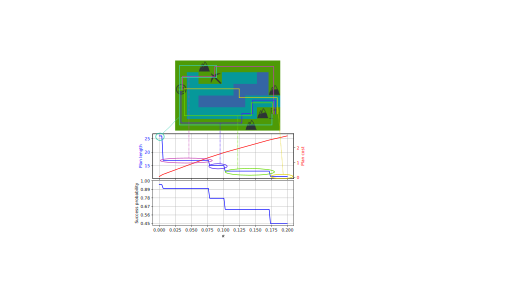
\includegraphics[width=0.85\textwidth]{terrain03alpha-plot}
	\caption{Solutions to an instance of the ``terrain'' problem using
			 $\alpha$-Cost-Transition-Likelihood Determinization with
			several values of $ \alpha $. }
	\label{fig:terrain03alpha-plot}
\end{figure}

Clearly, greater $\alpha$s result in more direct but riskier paths to the goal.
We can see that with $ \alpha > 0.175 $ the character happily accepts
swimming through deep water. On the other hand, low $ \alpha $ values are associated
to longer paths and safer plans. With $ \alpha = 0 $ the risk is minimal, since the
character puts himself
only in little danger to get the pickaxe through the shallow water. From that point on,
he slowly breaks his way to the target cell and going only through grass.


\paragraph{Example with Imagine domain:} We also present an example
of the application of $\alpha-Cost-Transition-Likelihood$ Determinization
in the recycling domain. We consider a very simple problem in which the robot
has to retrieve the PCB of a hard drive. The PCB is located at the bottom,
with four screws keeping it in place. Moreover, there is a connector from
the PCB to the motor axis. The PCB can be extracted either via levering
using the pliers, or bashing it with the hammer to loosen it and then letting
it fall. The hard drive is initially resting before the robot with its top
side facing upwards. Fig.~\ref{fig:imagine01alpha} shows that the effect
of the $\alpha$ parameter is the same as in the ``terrain'' example. Small
values lead to long but safe actions, while bigger values result in riskier
sequence. Notice, for instance, that the 4th plan uses the \texttt{bash} action
(the riskiest action in the repertoire) to quickly get rid of the 4 screws
that keep the PCB in place, and then the pliers to remove it from the drive.

\begin{figure}[p]
	\centering
	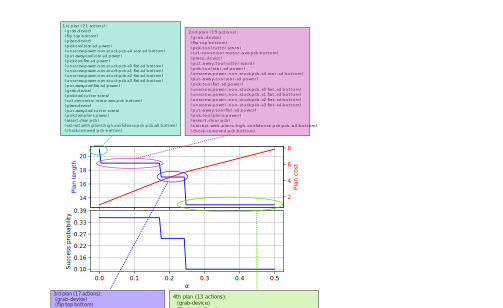
\includegraphics[width=\textwidth]{imagine01alpha}
	\caption{}
	\label{fig:imagine01alpha}. 
\end{figure}

\paragraph{Triangle Tireworld, an unfriendly domain:} Up to this point,
$\alpha$-Cost-Transition-Likelihood has worked as expected. However, it is
still somewhat vulnerable to domains with dead ends that are difficult to
avoid. This is the case of the Triangle Tireworld domain. Let us remember that
the goal is to reach the target node and avoiding getting stuck as result
of a flat tire. The probability of
getting a flat tire after moving is 50\%. It can be replaced if the car has
a spare. Spares are distributed among the different cells.

In this case, the $\alpha$ parameter has no influence and the planner
has no reason
to give preference to neither of the two outcomes because both have the
same probability and the same transition cost. In fact, the planner
will always suggest the shortest route, even
though this may not be the best choice. This is clear in Fig.~\ref{fig:ttwmap}.
While the safest route is going through the top of the triangle (the
\texttt{l-2-1} $\rightarrow$ \texttt{l-3-1} $\rightarrow$ \texttt{l-2-2} $\rightarrow$
\texttt{l-1-3} path), for the planner this plan has the same chances of succeeding as
the route that goes in a straight line from \texttt{l-1-1} to \texttt{l-1-3}.

This leads us to an interesting observation: even if the plans obtained
by a planner that operates in a determinized domain with $\alpha$ parameterized
costs are optimal, these do not induce the best policy. That is, repeatedly obtaining
the ``optimum'' plan (according to the $\alpha$-Cost-Transition-Likelihood criterion)
and executing the first action is not equivalent to executing
the optimum policy. The reason is somewhat subtle: even if two plans have the same
probability of succeeding and the same accumulated cost, the consequences of failing
one of the plans are not necessarily the same as the consequences of failing the second
one. Turning back to the Tireworld domain, we can see that if we get a flat tire going
through the top of the triangle, we can always pick one of the spares that are
distributed along the way and fix the tire. However, this is not the case in the
shortest route. In other words, the top route has more tolerance to failure than the
straight one.

Notice that we could easily manipulate the domain to make $\alpha-Cost-Transition-Likelihood$
work effectively in this particular case: we can alter the probabilities so that getting a
flat tire is more likely
than moving without hazard. Then, the cheapest plan with $\alpha = 0$ is the one that
always forces a flat tire at each movement, picks a new tire, and proceeds to the next
cell. Alternatively, we could artificially increase the transition cost of the outcome
of the move action in which the car does not get a flat tire.

This suggests a general approach to improve the robustness of $\alpha$-Cost-Transition-Likelihood
against dead-ends: if we are able to identify the most ``beneficial'' or ``desirable''
outcomes, we can artificially increment their transition cost so the planner does not get too
optimistic. However, automatically identifying such outcomes is not a trivial task in general.


\begin{figure}[tbp]
	\centering
	\includegraphics[width=0.5\textwidth]{ttw-p01-crop}
	\caption{}
	\label{fig:ttwmap}
\end{figure}

\section{Hindsight Determinization}

The last determinization method that we consider is not only a modification of the domain,
but also an algorithm to calculate a lower bound of the state-action utility (the same $ Q $
function that is used in many Reinforcement Learning algorithms) via repeated calls
to a deterministic planner.

Each time the action maker has to decide the next action, it calculates
an upper bound of the $ Q(s,a) $ for the current state and all the available action (or
an intelligently chosen subset of all the available actions). Let us call this
upper bound $ \hat{Q}(s,a) $. $ \hat{Q}(s,a) $ is assumed
to preserve the same ranking as the true $ Q $ function, and is calculated
averaging the negative length of several different plans traces that start with that action.
The longer the plans, the lower the $\hat{Q}$ score of that action for the given state. To obtain
different plans, the outcome of each action
is decided in \emph{hindsight} for each time step. For instance, for a given action with 5 outcomes,
the planner may decide that if the action is executed at time step 3, it will yield the fourth outcome.
In order to fix the outcomes in advance, they are sampled for each time step. The assignment of an
outcome for each action at each time step is called \emph{future}. If for a given action and future no
plan is found, then a penalty is applied to the $ \hat{Q} $ value of that action in order to make it less
appealing.

The method that we have outlined here has several advantages over the other determinization methods:
it makes the most of the probabilistic information about the outcomes; it invokes a planner several
times in order to base the decision on multiple possibilities; and it is very robust against
dead ends.
However, it also makes an intensive use of computational resources. Some improvements
have been suggested to reduce this intensive computation. One of them is computing
the $ \hat{Q} $ value of only a reduced set of actions. The set of actions is called
\emph{Probabilistically Helpful Actions}. One way to compute such set is to sample
several futures, plan for all of them, and retrieve the first action of each one. Another
improvement is to identify prefixes that are common in all the plans that start with the
selected action. These are usually deterministic actions and can be executed in sequence without
resorting to the Hindsight Optimization method for the intermediate states.

The original proposal only sets the outcomes of the actions up to
a certain horizon, so one must have an idea of the expected length of the plans before
setting this horizon. The authors of the method have modified the implementation of Fast Forward to
incorporate Hindsight Optimization using non-stationary action expansion. We propose
two method for performing Hindsight Optimization with out-of-the-box planners, using exclusively
PDDL features, and that does not fix the horizon of planning. More specifically, we use
a \emph{wheel of outcomes}, as shown inf Fig.~\ref{fig:hindsight-wheels}.

\begin{figure}[tbhp]
	\centering
	\begin{subfigure}[b]{0.4\columnwidth}
		\includegraphics[width=\textwidth]{hindsight-wheel-global}
		\caption{}
		\label{fig:wheel-global}
	\end{subfigure}
	
	\begin{subfigure}[b]{0.5\columnwidth}
		\includegraphics[width=\textwidth]{hindsight-wheel-local}
		\caption{}
		\label{fig:wheel-local}
	\end{subfigure}
	\caption{
		(a) Global time step. Each action as an outcome associated to each
			time step. The execution of any action makes the time step advance,
			potentially changing the available outcome for the rest of the actions.
		(b) Local action status. Each action has has associated an outcome for each
			of its internal statuses. The execution of an action makes the internal
			status advance, but it will not change the available outcome for the
            rest of the actions.
	}
	\label{fig:hindsight-wheels}
\end{figure}

The first method is the closest to the author's proposal. It is depicted
in Fig.\ref{fig:wheel-global}. The outcome that each action will
produce depends on the global time step.
However, time steps cycle as in a wheel, so the planner
is not constrained to plans that have lengths smaller than the horizon. What is more important,
this can be achieved using just PDDL:
\begin{itemize}
\item We introduce a \texttt{(current-timestep ?t)}.
\item Time steps are linked via several \texttt{(next-timestep ?t1 ?t2)} predicates. These define
the order of the time steps. The ``last'' time step is succeeded by the ``first'' one.
\item A predicate \texttt{(applicable-ai-oj ?t)} for each action $ a_i $ and outcome $ a_j $.
This predicate
tells, for every action, which outcome should be triggered at each time step.
\end{itemize}

Then, the domain is determinized in an All-Outcome fashion, but modifying the preconditions
so that an action outcome can be executed only when is applicable in the current time step.
The effects are also modified to make the time step advance. Since each action increments
the time step, the execution of an action alter the active outcome of the rest of the
actions.

The second method is similar, but it maintains a local status for each action rather than
a global one. The execution of an action modifies exclusively its own status, so the
planner is forced to trigger bad outcomes if it wants more beneficial effects from
the same action. The method is depicted in Fig.~\ref{fig:wheel-local}.

Fig.~\ref{fig:hindsight-hists} gives an idea of the power of the hindsight optimization method
for discriminating good actions from bad ones. It shows the negative $ \hat{Q} $ value
obtained from two states of the \texttt{rectangle-tireworld} and the \texttt{triangle-tireworld}
domains (therefore, the lower the value, the more appealing the action is).
We can observe that the issue that was present with $ \alpha $-Cost-Transition-Likelihood has been
mitigated.

In the first case (Fig.~\ref{fig:hist-rectangle}), the most promising action (and by a great
margin) is \texttt{(move-r n1 n1 n2)}. This makes sense when we understand the dynamics of the
rectangle tireworld domain: the car moves in a rectangular grid and can perform diagonal moves,
that allow to reach the goal much quicker, but sacrificing safety. The other three actions correspond
to diagonal movements.

In the second case (Fig.~\ref{fig:hist-triangle}), the most promising action is to pick a spare
from the current position. This makes sense. Let us remind that in this domain each displacement
action has associated a risk of getting a flat tire, so it is better to be prepared for the next
displacement, even if the car is in good state.

\begin{figure}[tbhp]
	\centering
	\begin{subfigure}[b]{0.56\columnwidth}
		\includegraphics[width=\textwidth]{rectangle-tireworld-hist}
		\caption{}
		\label{fig:hist-rectangle}
	\end{subfigure}
	~
	\begin{subfigure}[b]{0.30\columnwidth}
		\includegraphics[width=\textwidth]{triangle-tireworld-hist}
		\caption{}
		\label{fig:hist-triangle}
	\end{subfigure}
	\caption{
		(Negative) score of the assessed actions in a state of
		(a) the rectangle tireworld domain and
		(b) the rectangle tireworld domain.
	}
	\label{fig:hindsight-hists}
\end{figure}

\IfEq{\jobname}{\detokenize{root}}{}{\printbibliography}

\end{document}